\subsubsection{Displaymenu}
\label{subsubsec:Software_Displaymenu}

Das Bedienmenü am Display bietet dem Benutzer viele Freiheiten, was ein umfangreiches und möglichst intuitives Bedienkonzept erforderte. Folgende Einstellungen und Anpassungen können vom Benutzer vorgenommen werden:


\begin{itemize}
\item Getränkeauswahl gemäss Bild oder Listenansicht
\item Zutatenabfrage
\item Bearbeitung von bereits existierenden Cocktails
\item Erstellen neuer Cocktails 
\item Individuelle Zusammenstellung und Positionierung von Flüssigkeiten
\item Zuweisung eines Getränkes zu einem RFID-Tag
\item Anzeige einer Maschineninfo
\item individuelle Beleuchtung der Maschine
\item Maschinen Reinigungsmodus
\end{itemize}

Im folgenden wird auf die gesamte Menüstruktur eingegangen und erklärt, wie diese zu bedienen ist.

\textbf{Hauptansicht}\\
In der Hauptansicht gemäss Abbildung \ref{fig:DisplayHauptmenu} wird die Getränkeauswahl getroffen. Dabei gibt es zwei verschiedene Auswahlmöglichkeiten. Mit den Pfeiltasten nach links oder rechts kann ein Getränk aus der Maschine ausgewählt werden. Es wird dabei immer der Getränkename und eine dazugehörige Abbildung angezeigt, damit dem Kunden der Cocktail auch schmackhaft gemacht werden kann. Will man schneller suchen, so kann man mittels \flqq Liste\frqq~eine Listenansicht öffnen, wobei man mit den Pfeiltasten nach oben und unten scrollen und den gewünschten Cocktail auswählen kann. Wird eine Auswahl getroffen, so gelangt man zurück in die Hauptansicht und der gewählte Cocktail erscheint mit dem dazugehörigen Bild. Mit \flqq Zurück\frqq~gelangt man ebenfalls zurück in die Hautansicht. Es gibt auch Filtermöglichkeiten. Auf der rechten unteren Seite des Display's kann per Klick entschieden werden, ob nur alkoholische, alkoholfreie oder alle Cocktails angezeigt werden. Hat man ein Getränk gefunden und möchte wissen was sich darin befindet und wie viel, so kann man mittels Klick auf \flqq Zutaten\frqq~ein Fenster öffnen, welches einem anzeigt was und wie viel davon sich darin befindet. Möchte man Einstellungen vornehmen, so gelangt man mittels \flqq Menü\frqq~in das Maschinenmenü.

\begin{figure}[h!]
	\centering
	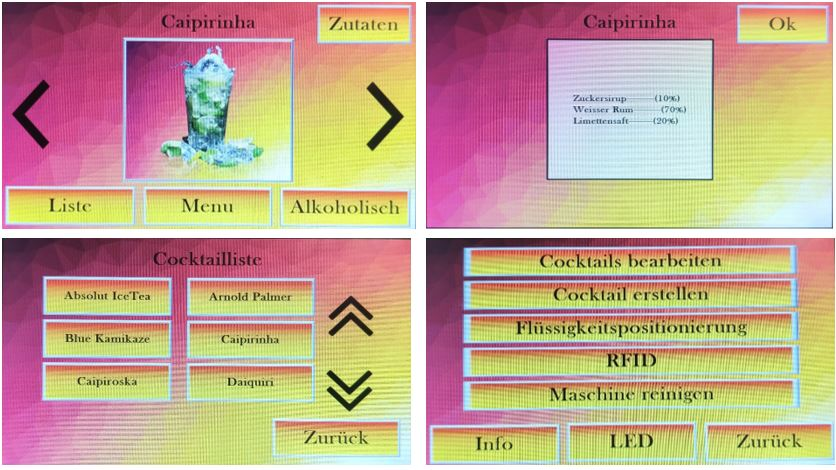
\includegraphics[width=\textwidth]{graphics/DisplayHauptmenu}
	\caption{Hauptansicht der Menüstruktur des Display's}
	\label{fig:DisplayHauptmenu}
\end{figure}

\textbf{Getränkeauslösung}\\
Wurde die Auswahl für ein Getränk getroffen, so kann man mittels Klick auf das Bild das Getränk auslösen. Dabei gelangt man in eine Abfrage, welche dem Kunden die Wahl lässt, ob er gerne 3dl oder 5dl haben möchte. Mit \flqq Abbrechen\frqq~gelangt man in die Hauptanzeige zurück. Bei Klick auf den entsprechenden Button 3dl oder 5dl wird die gewünschte Grösse des Getränks ausgelöst und am Bildschirm erscheint ein kleiner Text, welcher einem das Warten versüsst. Dazu muss natürlich ein Glas vom Kunden auf den Schlitten gelegt werden. Der Schlitten befördert nun das Glas zu den einzelnen Positionen und füllt es dort ab. Sobald das Getränk fertig ist, fährt der Schlitten an die Ausgangsposition zurück und es wird am Bildschirm angezeigt, dass das Getränk nun fertig ist. Es erscheint danach erneut der Hauptbildschirm und es kann von neuem gestartet werden. Wird während des Erstellungsvorgangs auf \flqq Abbrechen\frqq~gedrückt, so wird der Prozess abgebrochen und das Display zeigt dies an. In Abbildung \ref{fig:DisplayAusloesen} sind die dazugehörigen Bildschirme zu sehen.

\begin{figure}[h!]
	\centering
	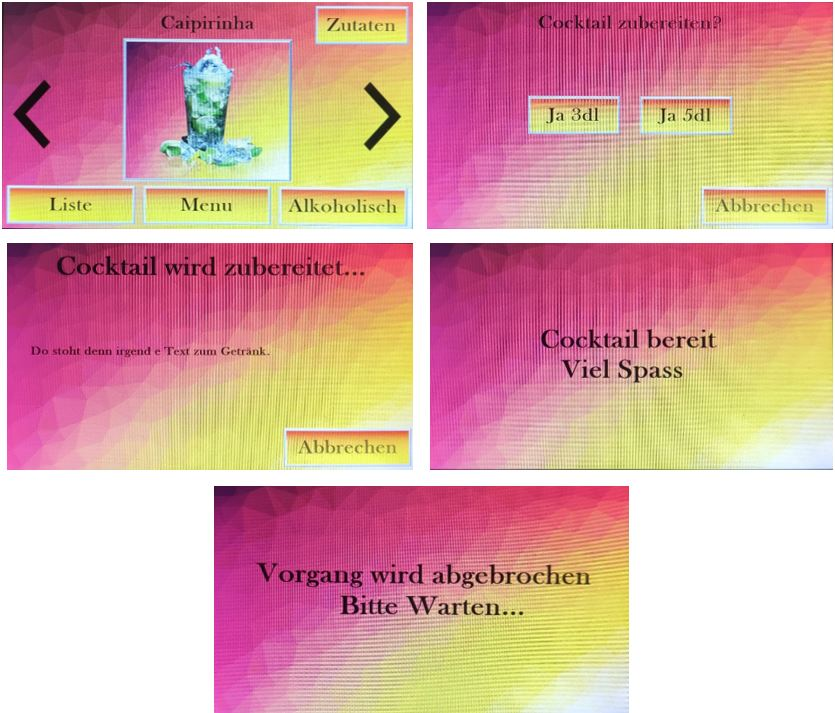
\includegraphics[width=\textwidth]{graphics/DisplayAusloesen}
	\caption{Auslösevorgang der Menüstruktur des Display's}
	\label{fig:DisplayAusloesen}
\end{figure}

\newpage

\textbf{Maschineninfo und LED-Beleuchtung}\\
Im Maschinenmenü kann unten links eine Info angezeigt werden, welch dem Kunden eine Information gibt, wer diese Maschine gebaut hat und wieso. Die Maschine verfügt über eine eigene Beleuchtung mittels RGBW-LED's. Diese kann vom Kunden individuell eingestellt werden. Klickt man auf \flqq LED\frqq~, so erscheint das Beleuchtungsmenü. in diesem Menü kann die Beleuchtung entweder auf weiss, Rainbow oder Custom eingestellt werden. Wird auf \flqq Weiss\frqq~gedrückt, so leuchtet die Maschine weiss. Bei \flqq Rainbow\frqq~, was standartmässig eingestellt ist, werden die Farben langsam abwechselnd durchgespielt. Wird \flqq Custom\frqq~gedrückt, so können mittel Schieberegler eigene Farben eingestellt werden. Am Anfang stellen sich die Schieberegler auf die zuvor eingestellte Farbe ein. So kann auch mittels Rainbow eine Farbe belassen werden, wenn einem eine Farbe sehr gut gefällt. Wird \flqq Zurück\frqq~betätigt, so gelangt man erneut in das Maschinenmenü. Die dazugehörigen Menübildschirme sind in Abbildung \ref{fig:DisplayInfoLed} zu sehen.

\begin{figure}[h!]
	\centering
	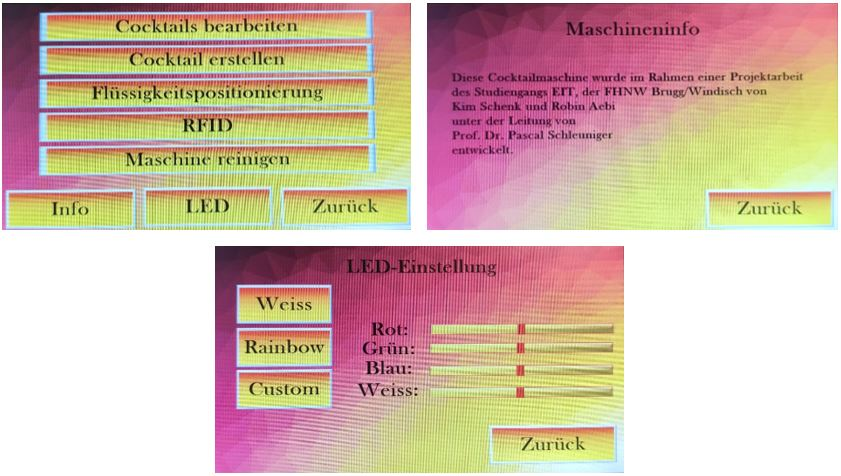
\includegraphics[width=\textwidth]{graphics/DisplayInfoLed}
	\caption{Infomenü und LED Einstellungen der Menüstruktur des Display's}
	\label{fig:DisplayInfoLed}
\end{figure}

\textbf{Cocktails bearbeiten}\\

\begin{figure}[h!]
	\centering
	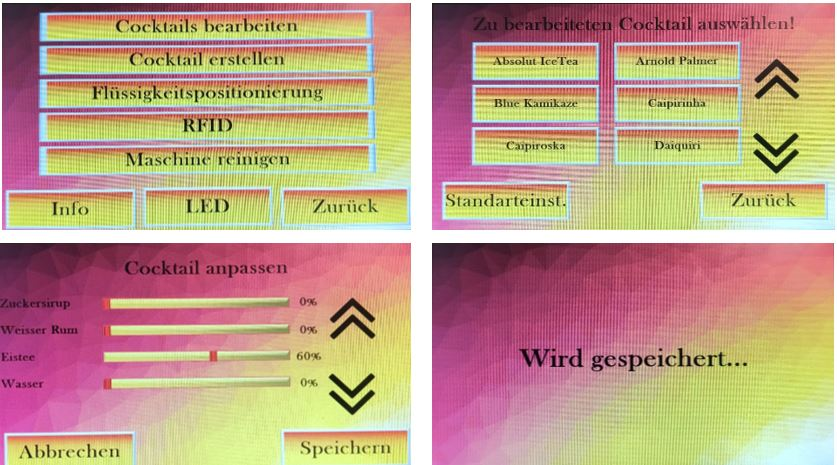
\includegraphics[width=\textwidth]{graphics/DisplayBearbeiten}
	\caption{Cocktail Bearbeitungsmenü der Menüstruktur des Display's}
	\label{fig:DisplayBearbeiten}
\end{figure}

\begin{figure}[h!]
	\centering
	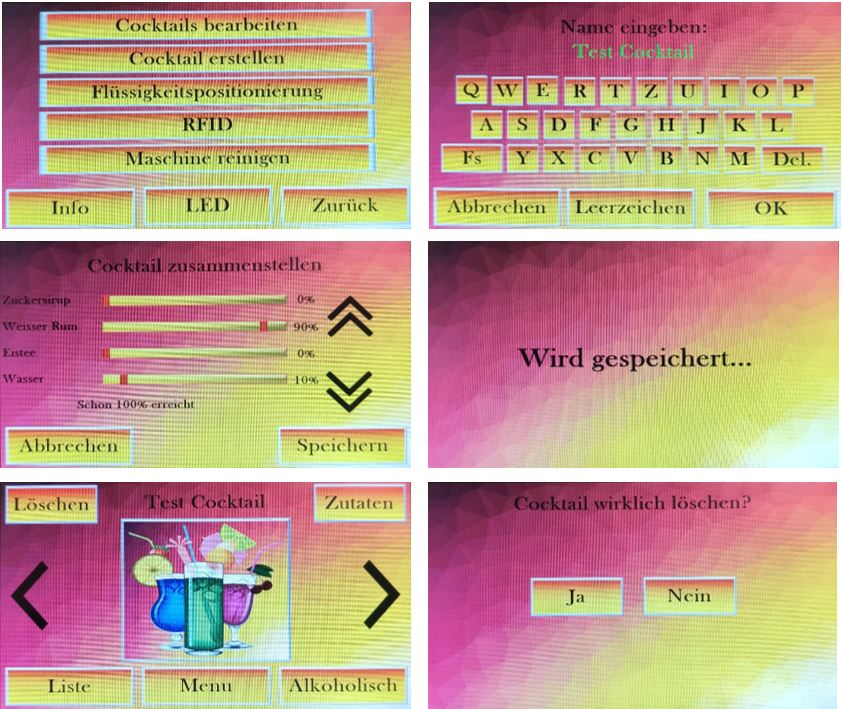
\includegraphics[width=\textwidth]{graphics/DisplayErstellen}
	\caption{Cocktail Erstellungsmenü der Menüstruktur des Display's}
	\label{fig:DisplayErstellen}
\end{figure}

\begin{figure}[h!]
	\centering
	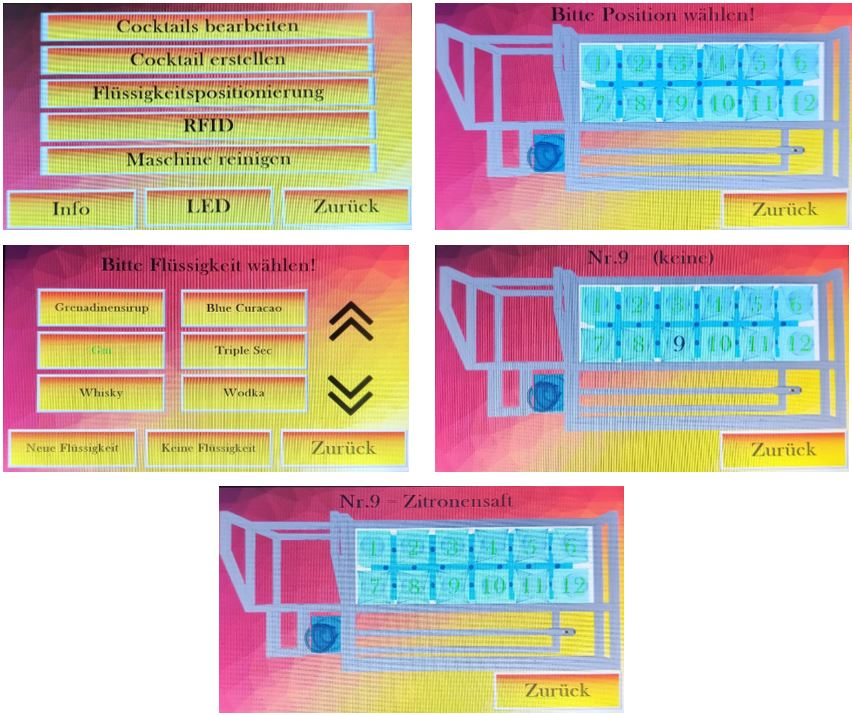
\includegraphics[width=\textwidth]{graphics/DisplayPositionierung1}
	\caption{Flüssigkeitspositionierung der Menüstruktur des Display's}
	\label{fig:DisplayPositionierung1}
\end{figure}

\begin{figure}[h!]
	\centering
	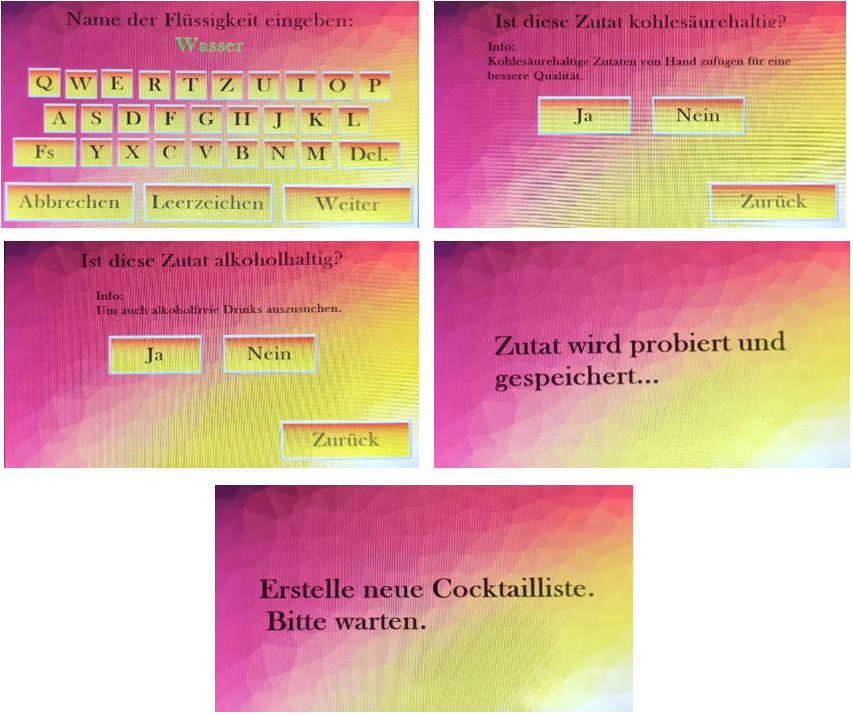
\includegraphics[width=\textwidth]{graphics/DisplayPositionierung2}
	\caption{Flüssigkeitserstellung der Menüstruktur des Display's}
	\label{fig:DisplayPositionierung2}
\end{figure}

\begin{figure}[h!]
	\centering
	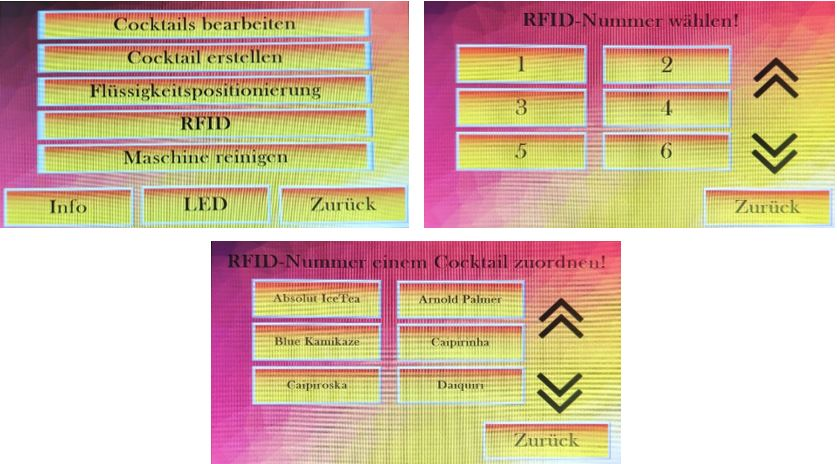
\includegraphics[width=\textwidth]{graphics/DisplayRFID}
	\caption{RFID-Zuweisung der Menüstruktur des Display's}
	\label{fig:DisplayRFID}
\end{figure}

\begin{figure}[h!]
	\centering
	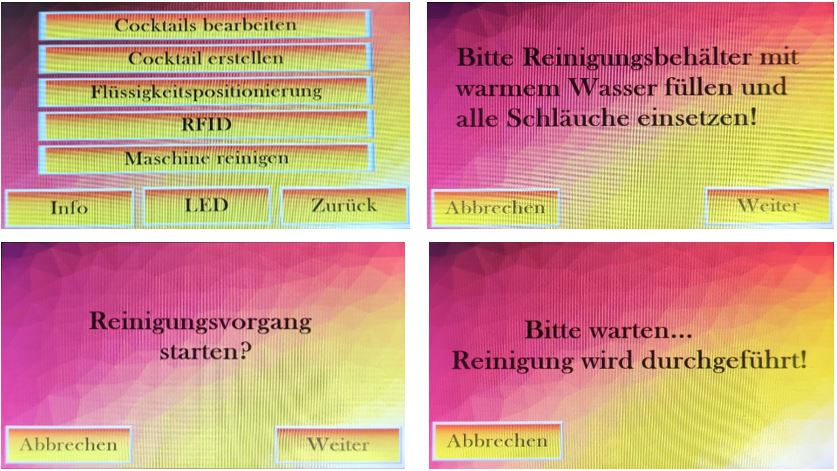
\includegraphics[width=\textwidth]{graphics/DisplayReinigen}
	\caption{Reinigungsmodus der Menüstruktur des Display's}
	\label{fig:DisplayReinigen}
\end{figure}

\newpage


